\documentclass[journal,twoside]{IEEEtran}
\IEEEoverridecommandlockouts
% The preceding line is only needed to identify funding in the first footnote. If that is unneeded, please comment it out.
\usepackage{cite}
\usepackage{hyperref}
\usepackage{natbib}
\usepackage{booktabs}
\usepackage{diagbox}
\usepackage{threeparttable}
\usepackage{amsmath,amssymb,amsfonts}
\usepackage{algorithmic}
\usepackage{graphicx}
\usepackage{textcomp}
\usepackage{xcolor}
\makeatletter
\def\UrlAlphabet{%
      \do\a\do\b\do\c\do\d\do\e\do\f\do\g\do\h\do\i\do\j%
      \do\k\do\l\do\m\do\n\do\o\do\p\do\q\do\r\do\s\do\t%
      \do\u\do\v\do\w\do\x\do\y\do\z\do\A\do\B\do\C\do\D%
      \do\E\do\F\do\G\do\H\do\I\do\J\do\K\do\L\do\M\do\N%
      \do\O\do\P\do\Q\do\R\do\S\do\T\do\U\do\V\do\W\do\X%
      \do\Y\do\Z}
\def\UrlDigits{\do\1\do\2\do\3\do\4\do\5\do\6\do\7\do\8\do\9\do\0}
\g@addto@macro{\UrlBreaks}{\UrlOrds}
\g@addto@macro{\UrlBreaks}{\UrlAlphabet}
\g@addto@macro{\UrlBreaks}{\UrlDigits}
\makeatother
\def\BibTeX{{\rm B\kern-.05em{\sc i\kern-.025em b}\kern-.08em
    T\kern-.1667em\lower.7ex\hbox{E}\kern-.125emX}}
\newcommand{\tabincell}[2]{\begin{tabular}{@{}#1@{}}#2\end{tabular}}
\pagestyle{headings}
\markboth{Bioinformatics. Specialty  Innovation  and  Entrepreneurship  Training 2021}
{Zhao. A Support Vector Machine Method for Prediction of Eukaryotic Genetic Splice Sites (June 2021)}
\begin{document}

\title{A Support Vector Machine Method for Prediction of Eukaryotic Genetic Splice Sites \\
}

\author{\IEEEauthorblockN{1\textsuperscript{st} Ziwen Zhao} \\
\IEEEauthorblockA{\textit{College of Life Science and Technology} \\
\textit{Huazhong University of Science and Technology}\\
Wuhan, China \\
justn582@gmail.com}
}

\maketitle

\begin{abstract}
Splice sites are a vitally important gene sequence pattern amongst the functional sites inside a eukaryotic gene. However, splice site prediction does not come easy thanks to the extreme complexity of human genome. In this paper, a discriminant analysis method to predict splice site patterns using a support vector machine is proposed, which is an effective, high-accuracy approach for splice site prediction in comparison with some other models on the renowned Kulp \& Reese human genome dataset, during which we achieve excellent results on several different metrics. We proved that 4D-polynomial SVM is the best model for splice site prediction tasks among all the predictors we mentioned and estimated. The source code is available on GitHub and can be obtained from \url{https://github.com/Newiz430/SplicePredictor}. 
\end{abstract}

\begin{IEEEkeywords}
splice site, support vector machine, discriminant analysis, kernel function, grid searching
\end{IEEEkeywords}

\section{Introduction}\label{1}
\IEEEPARstart{G}{ene} finding by computational methodologies, the foundation for all further investigation in functional genomics, has attracted considerable research attention since the 20\textsuperscript{th} century \cite{burge1997prediction}. With the thriving of functional genomics after the completion of Human Genome Project (HGP), functions of the elements of eukaryotic gene sequences were beginning to surface. Researchers came to realize that DNA sequences, other than genes, contain a huge amount of information, most of which is correlated with the structural features of nucleic acids and in general determines the DNA - protein, or DNA - RNA interactions. Such information is mostly provided by a variety of functional sites (i.e. sequence motif). The splice sites are a vitally important eukaryotic gene sequence pattern amongst all these sites. As terminal points of RNA splicing, splice sites label the junction of transcript exons and introns, assisting biologists in identifying and positioning the coding sequence within a gene. Splicing, itself, also influences the structure and function of genes, which makes genes more ``modular'', allowing new combinations of exons to be created during evolution. Furthermore, new exons can be inserted into old introns, creating new proteins without disrupting the function of the old gene \cite{clancy2008rna}. Hence the discovery and prediction of splice sites are of great significance for genetic selective expression research. 

\begin{figure}[htbp]
\centerline{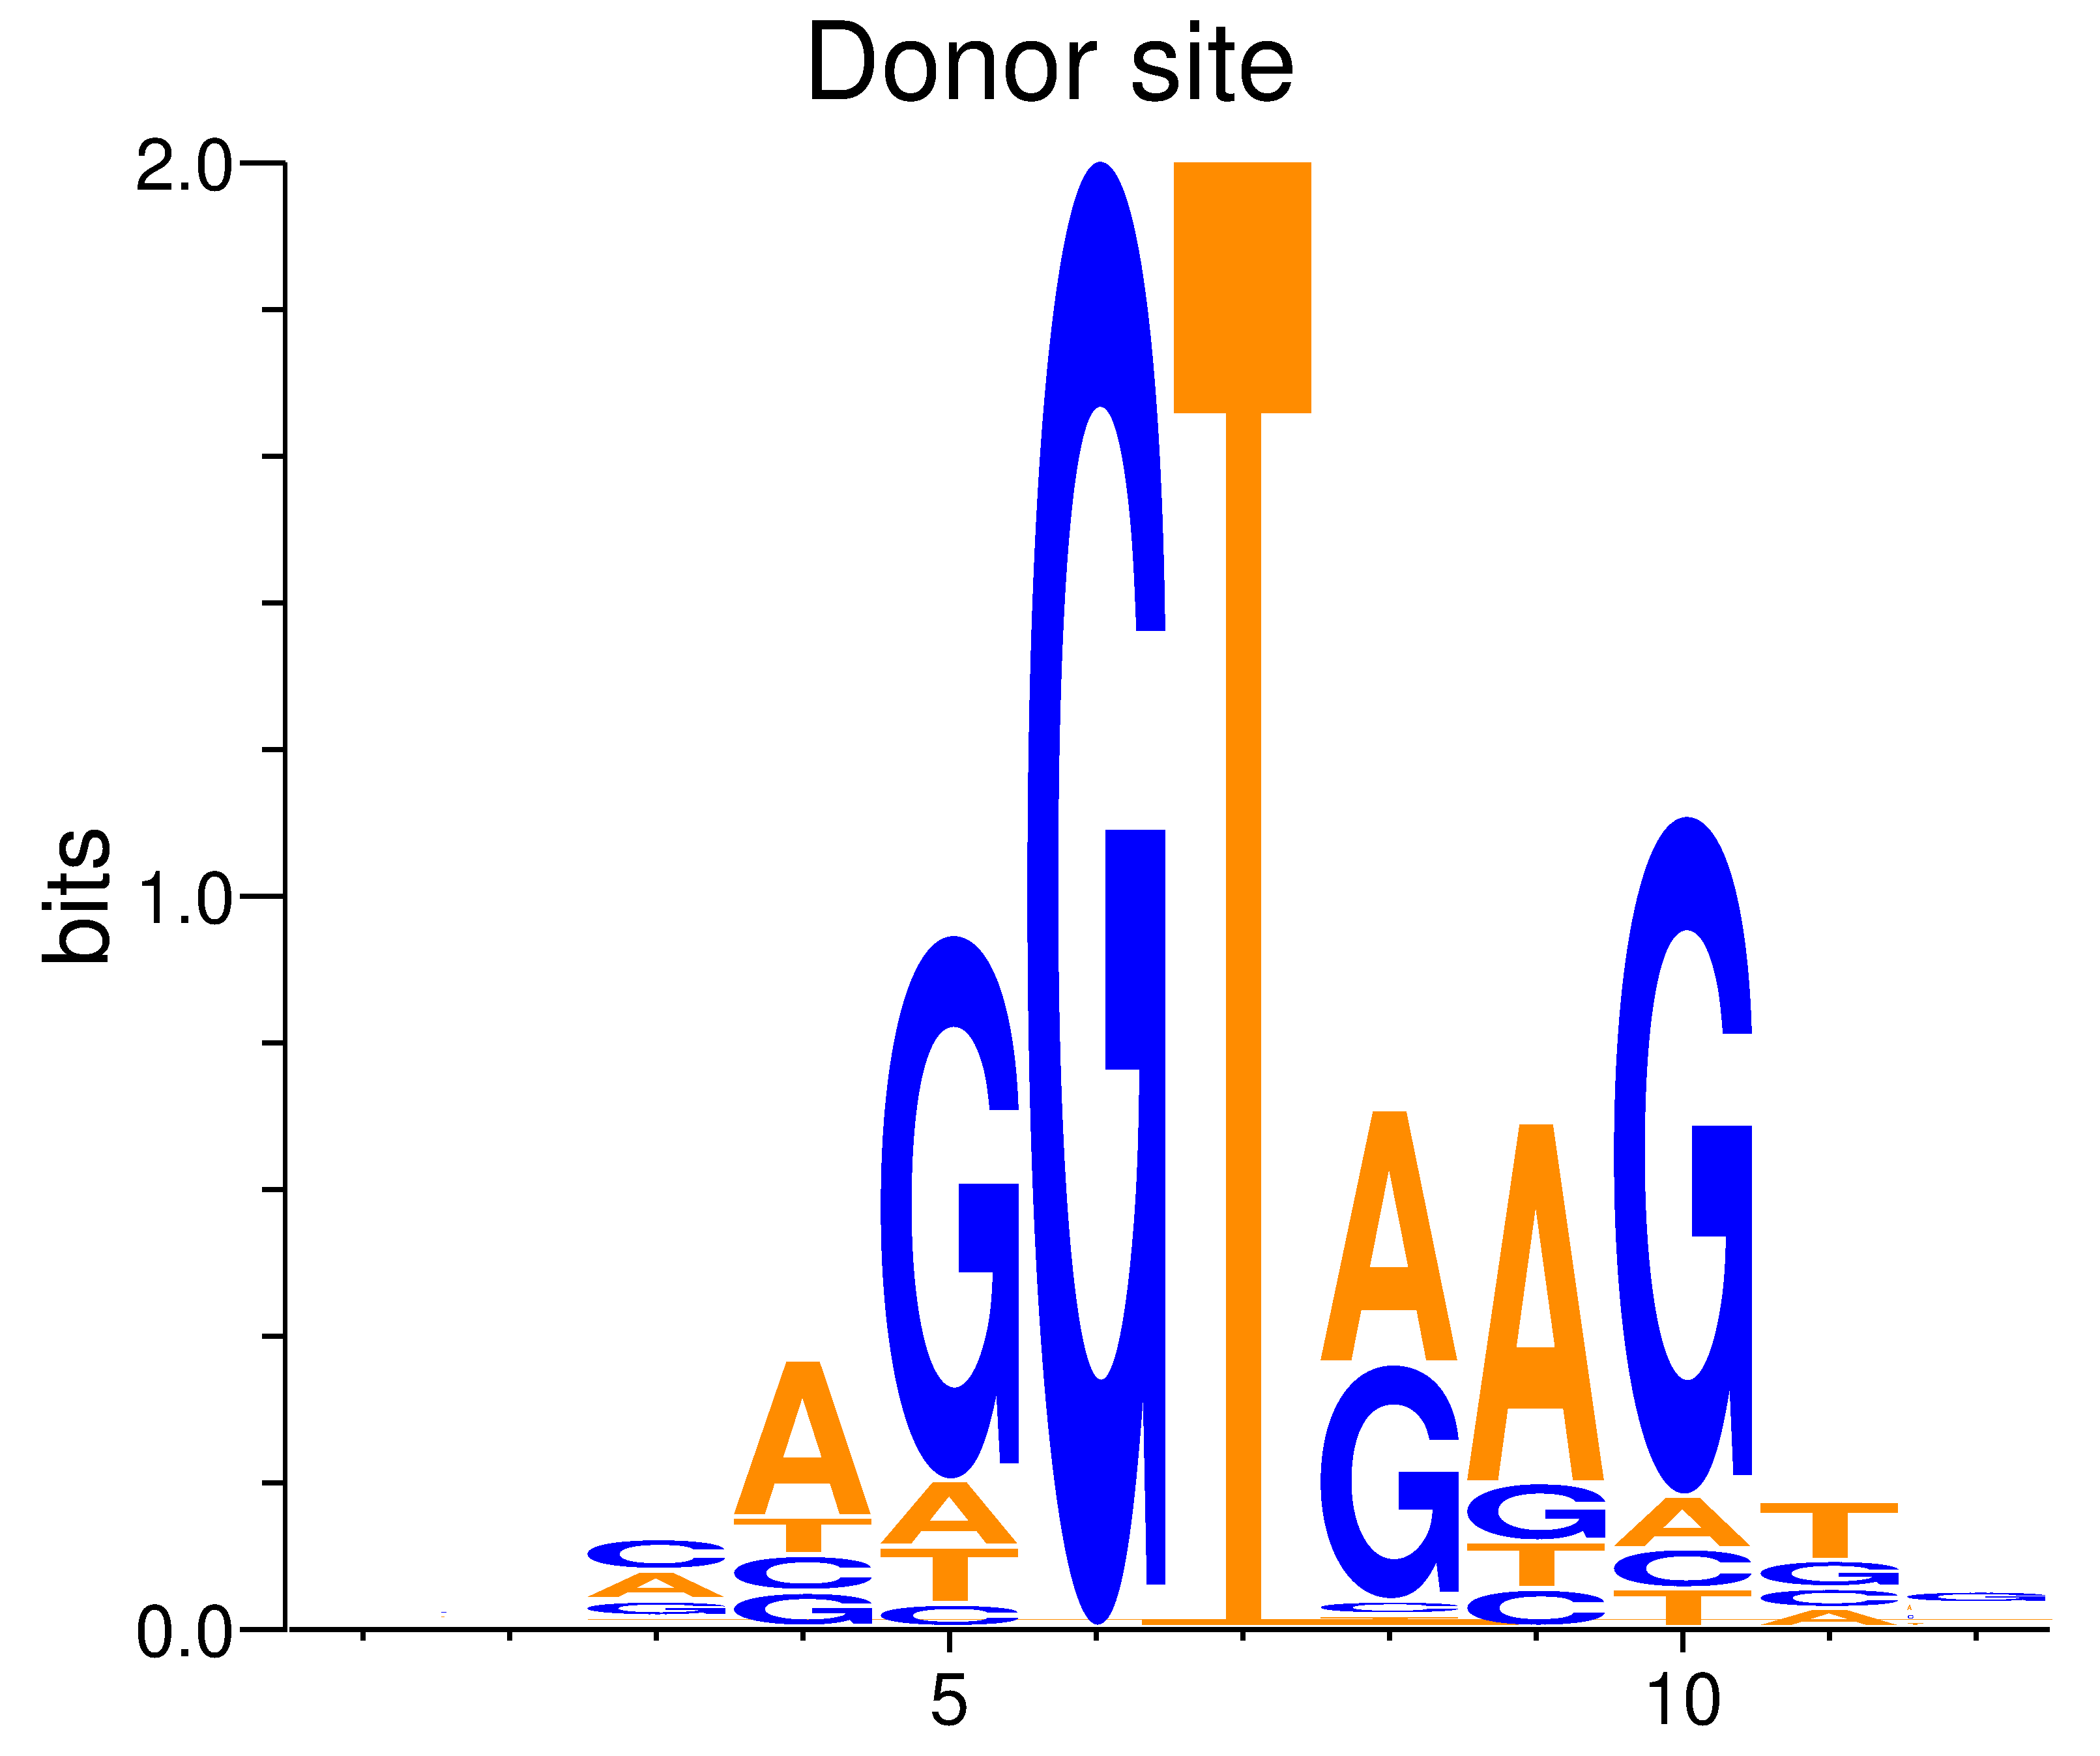
\includegraphics[scale=0.85]{Pics/donor_logo.png}}
\centerline{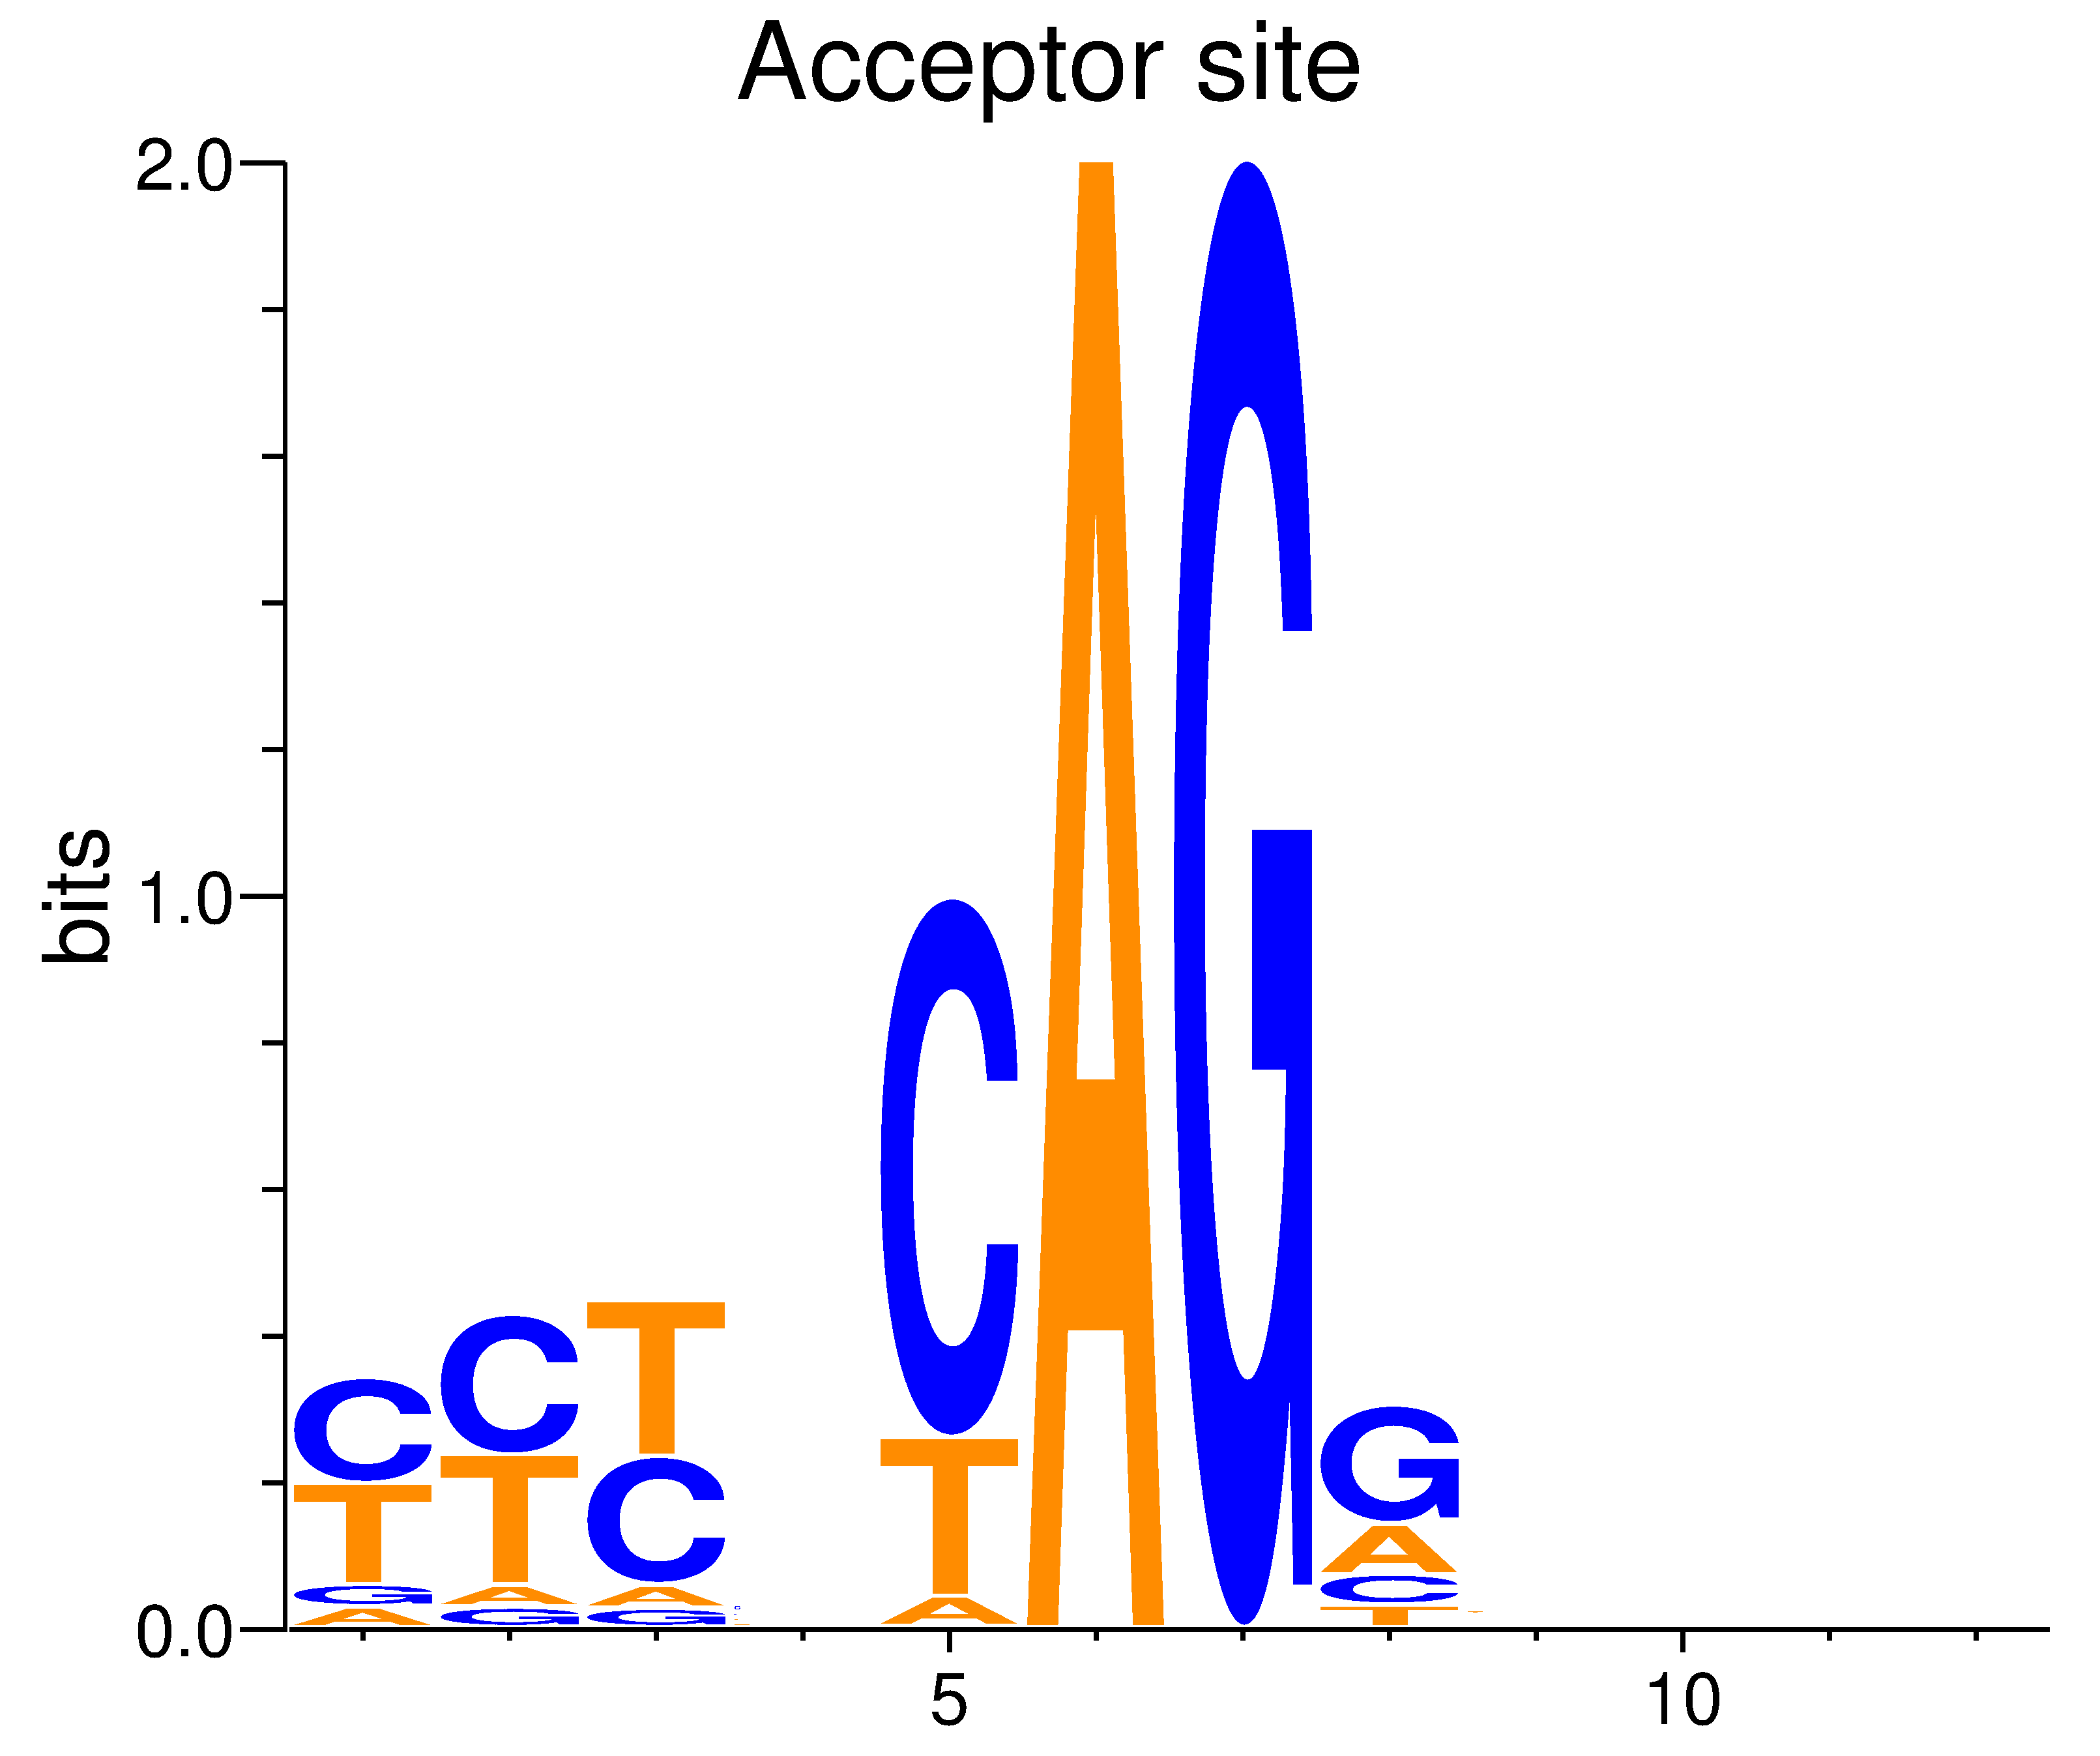
\includegraphics[scale=0.85]{Pics/acceptor_logo.png}}
\caption{Base distribution represented as sequence logos \cite{schneider1990sequence} for eukaryotic gene splice sites (5 upstream sites, 2 conservative sites \& 5 downstream sites): \textbf{top}, donor site; \textbf{bottom}, acceptor site. The most conserved sites is revealed within logo pictures: for donor sites, GT (6, 7); acceptor sites, AG (6, 7). Despite these two, distribution of adjacent sites (5, 8, 9, 10 for the donor, 5 for the acceptor) appear to have some consistency, too. The polypyrimidine tract can also be observed upstream of the acceptor site (1, 2, 3). The information content at a certain point $R_i$ is given by $R_i = \log_24 - (H_i + e_n)$ where $H_i = -\sum\limits_{i=1}^4{P_i(\log_2{P_i})}$ is the Shannon entropy \cite{shannon1948mathematical}, using bit as the basic unit. Higher the bits, higher the relative frequency of that base \cite{schneider1986information}. }
\label{fig1}
\end{figure}

A splice site locates in the edge of an intron, including a donor site (5' end of the intron) and an acceptor site (3' end of the intron). As a typical sequence motif, the donor site includes an almost invariant sequence GU at the 5' end of the intron, within a larger, less highly conserved region. The splice acceptor site at the 3' end terminates the intron with an almost invariant AG sequence \cite{black2003mechanisms}.  Some sections of the intron foretell the positions of these two sites. For example, a fragment of sequence upstream of the acceptor consisting of cytosines and thymines, which is called a polypyrimidine tract \cite{lodish2008molecular}. Fig. \ref{fig1} shows the base distributions adjacent of the splice donor sites and acceptor sites. 

As a matter of fact, accurate prediction does not come easy thanks to the extreme complexity of human genome. On one hand, the number and length of exons and introns in a eukaryotic gene exhibit great uncertainty. One eukaryotic gene contains 5.48 exons with 30 - 36 bps long on average. While the longest exon in the human genome is 11555 bp long, several exons have been found to be only 2 bp long \cite{sakharkar2004distributions}. On the other, the existence of alternate splicing make it harder to predict \cite{black2003mechanisms}. In this paper, we apply a feasible lightweight computational approach for gene functional site finding to predict eukaryotic gene splice sites, and prove its accuracy and high efficiency. 

\subsection{Related Work}\label{1.1}

Several typical computational methods that attempt to predict eukaryotic splice sites from unknown gene sequences (i.e. \textsl{ab initio} prediction) have been proposed previously. 

Frequency-based methods count the nucleotide frequencies of each site via multiple sequence alignment, etc. and work out the log-odds ratio to compare and find conservative sections in the alignment results. Rodger, et al. (1983) \cite{staden1984computer} proposed a computational model using a weight matrix to represent each type of recognition sequence. A weight matrix is a two dimensional array of values that represent the score for finding each of the possible sequence characters at each position in the target signal. The Weight Matrix Model (WMM) now becomes deprecated owing to its poor accuracy and its independence assumption, that is, WMM only takes point-wise base distribution into consideration, regardless of the potential dependence between adjacent points which is more conformable to the realistic situations. Zhang et al. (1993) \cite{zhang1993weight} optimized the weight matrix to weight arrays which take into account the correspondence between current position and an adjoining position, which is certified conducive to promote accuracy of splice site prediction, but this is still relying on the hypothesis that the intrinsic interdependency only exists between adjacent sites. To deal with the predicament, Burge, et al. (1997) \cite{burge1997prediction} explored a maximal dependence decomposition method and developed the software GENSCAN which identifies complete exon / intron structures of genes, which performs better but still generates many false positive results. 

Bayesian methods are ones that consider long range dependency among nucleotide sequences. Chen, et al. (2005) \cite{chen2005prediction} proposed a method using dependency graphs and its expanded form - Bayesian Network to fully capture the intrinsic interdependency between base positions in a splice site. The entire model, including the DAG structures and conditional probabilities, is learned \textsl{ab initio} from a training set. However, with astronomical computation complexity and model training difficulty, the performance of Bayesian models is not in keeping with them. 

Supervised learning methods learn a model from existing training set which is able to identify the most effective pattern automatically. Ryen et al. (2008) \cite{ryen2008splice} introduced the artificial neural network (ANN) in this area and trained the model with backpropagation, which can make predictions without prior knowledge of any sensor signals. Accurate and efficient learning approaches it is, supervised learning methods are heavily dependent on the mass and quality of training sets. Models may not be improved and a computational resource waste may happen when an unbalanced dataset or one with too many noises is provided. Moreover, neural networks acquire a suitable framework and initial hyperparameters. 

\subsection{Contributions}\label{1.2}

In this work, we propose a discriminant analysis method to predict splice site patterns using a support vector machine, the principle of which is to map samples linear-inseparable in the primal n-dimension feature space to a higher dimension feature space where they become linear-separable by mathematical transformations. Our contributions are listed as follows. 

\begin{itemize}
\item We implemented the support vector machine by Scikit-Learn, Python \cite{pedregosa2011scikit} using the given KR set and estimated its performance on the BG set, referring to the existing experiment by Duan, et al. (2008) \cite{duan2008position}.
\item We assessed the influence of various kernel functions to the SVM model. 
\item We did a comparison study among WMM, WAM, Bayesian network and ours to prove the superiority of our model. 
\end{itemize}

\begin{figure*}[htbp]
\centerline{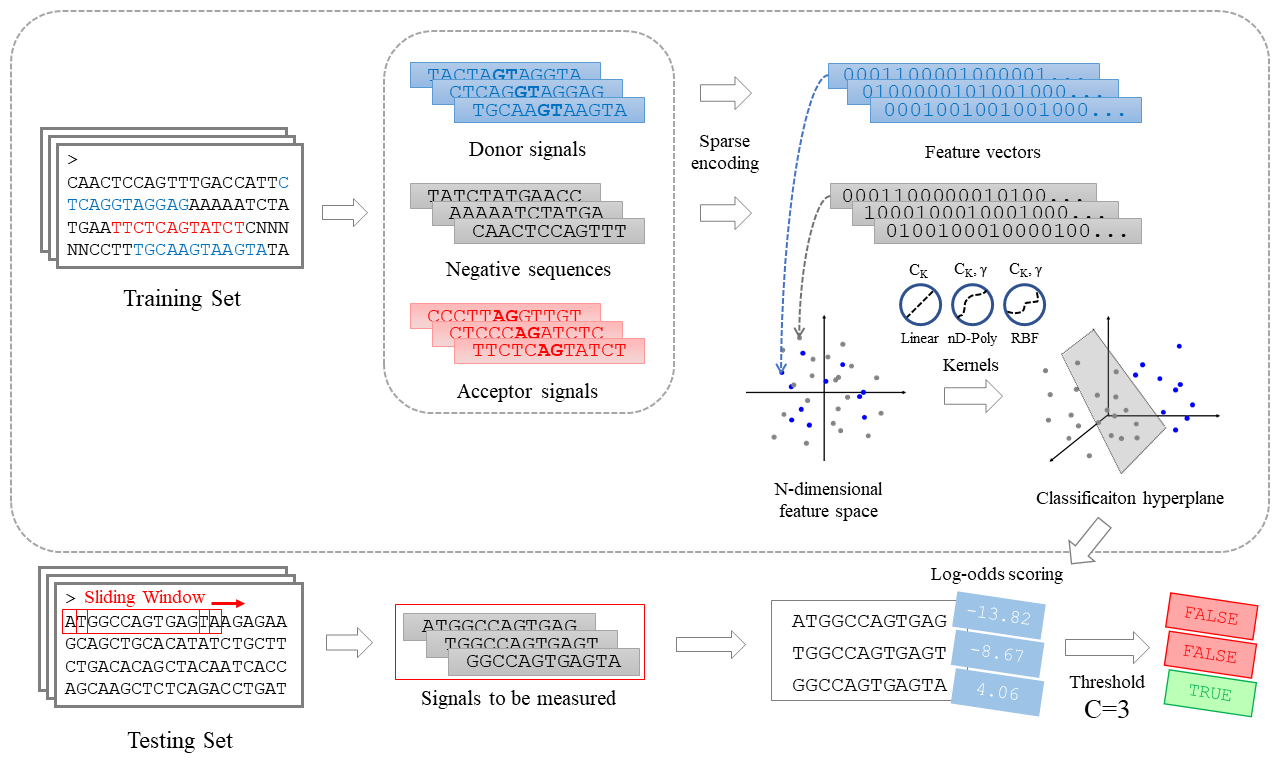
\includegraphics[scale=0.5]{Pics/SVM.png}}
\caption{Overall architecture of the support vector machine splice predictor. We use the training set to train a SVM model by the following steps: extracting positive site signals \& randomly choosing negative signals, encoding the signals into n-dimensional one-hot vectors, choosing an appropriate kernel and standardization coefficient $C_K$ (also $\gamma$ if RBF or polynomial kernel is used, $d$ for degree of polynomial kernel) and learning a decision hyperplane to split positive and negative sample points. SVM is used for splice site prediction by these steps: extracting testing sequences of same length by window-sliding, scoring the sequences position-wise with the decision hyperplane, calculating the binary log-odds scores, and comparing them with a given threshold to make final judgment. }
\label{fig2}
\end{figure*}

\section{Methods}\label{2}

Our method is illustrated in Fig. \ref{fig2}, which mainly contains two parts. A decision hyperplane is trained which separates the training data at the ``training'' step, and sequences of the testing set are scored by the decision hyperplane at the ``predicting'' step. See below for more detailed presentation. 

\subsection{Hypothesis}\label{2.1}

We assume conservation around the functional splice sites through the entire experiment. This is the fundamental premise for fundamental site finding methods. As for data, we assume that everything about the splice site pattern remained unknown (including the obligatory sites GT / AG) until we dug them out, in order to guarantee the generality of our model, since our aim is to make it possible to branch out to other unidentified functional sites. 

\subsection{Data Extraction}\label{2.2}

Dash et al. (2001) \cite{dash2001modeling} found in predicting splice sites by a Bayesian network that it achieves better performance when both of the upstream and downstream feature lengths are greater than 15. With a view to simplifying model and decreasing the computation, we choose 5 upstream sites and 7 downstream sites of intron / exon junctions to form 12 nt long signal sequences from the primary training set. We abandon sequences containing ambiguous bases, whose correspondence with the splice sites we consider inapparent. The training set provides 2,381 donor signals and 2,381 acceptor signals. As for negative samples, Chen, et al. \cite{chen2005prediction} used pseudo splice sites as false data, extracted by searching for negative sample sequences with $P_{+1}P_{+2} = \text{GU / AG}$ whereas, according to the splice site hypothesis above, We randomly selected about 5,000 sites in sections which do not intersect with all donor and acceptor sites, and combined with positive ones to get actual training dataset, the positive-negative ratio of which is about 1:2. Additionally, we export sequences with the same length by window sliding from the primal testing set and build the actual testing set in a positive-negative ratio of 1:20. 

For the data imbalance of negative sites versus positive ones, a feasible approach was proposed by Wen, et al. (1999) \cite{fang1999splice} who split the SVM classifier into 3 sub-classifiers which use a shared set of positive samples but different sets of negative samples, and picked the lowest prediction score on the testing set among all 3 scores generated by sub-classifiers as the final result. Instead we use a much simpler method which adds specific attention weights to the classes, forcing SVM to pay more attention to the minor positive samples. 

\subsection{Encoding}\label{2.3}

Next, we encode the filtered sequence samples. We choose the simplest encoding approach which based only on the composition of bases at every site. A, C, G and T bases are encoded as one-hot variables $[1, 0, 0, 0]$, $[0, 1, 0, 0]$, $[0, 0, 1, 0]$, $[0, 0, 0, 1]$, which are concatenated in order to form one $4\lambda$ long vector. Results show unexpectedly that SVM with this simple encoding method performs well in the prediction task. 

\subsection{Fitting a Hyperplane}\label{2.4}

As Cortes and Vapnik (1995) \cite{cortes1995support} proposed previously, firstly we need to make the sample vectors $\textbf{X}$ linear-separable inside the feature space before training an optimal hyperplane for classification (a ``plane'' with far more than 2 dimensions), that is, we use a generalized linear discriminant function $f(\textbf{X})$ as the decision function, which is defined as: 
\begin{align}
f(\textbf{X}) & = \textbf{W} \cdot \varphi(\textbf{X}) + b \notag \\
& = \sum\limits_{i=1}^N \alpha_i y_i (\varphi(\textbf{X}_i) \cdot  \varphi(\textbf{X})) + b
\label{eq1}
\end{align}
where vector $\textbf{W}$ determines the direction of the hyperplane and b determines the distance between the hyperplane and the origin. 

SVM lowers the difficulty of hyperplane learning by substituting a kernel function $K(\textbf{X}_i, \textbf{X})$ for the inner product of the mapping function $\varphi(\cdot)$ which should have been implemented. The discriminant function of an SVM is given as follows: 
\begin{align}
f(\textbf{X}) & = \textbf{W} \cdot \varphi(\textbf{X}) + b \notag \\
& = \sum\limits_{i=1}^N \alpha_i y_i K(\textbf{X}_i, \textbf{X}) + b
\label{eq2}
\end{align}

Kernels determines the high-dimensional space the features to be mapped to, so the first step is to select a proper kernel for SVM. There are 3 frequently used kernels: linear kernel, radial basis function kernel (RBF kernel, also called Gaussian kernel) and polynomial kernel, the forms expressed as:
\begin{equation}
\begin{cases}
K_\text{linear}(\textbf{X}_i, \textbf{X}_j) = \textbf{X}_i \cdot \textbf{X}_j \\
K_\text{rbf}(\textbf{X}_i, \textbf{X}_j) = \exp(-\gamma\| \textbf{X}_i - \textbf{X}_j \|^2) \\
K_\text{poly}(\textbf{X}_i, \textbf{X}_j) = (\gamma (\textbf{X}_i \cdot \textbf{X}_j)+r)^d
\end{cases}
\label{eq3}
\end{equation}
where $\gamma = \frac{1}{2\sigma^2}$ is the kernel coefficient. In our work, we applied all 3 kernels on one SVM, finetuning the hyperparameters for each, to find out the one bringing the best predicting performance. See \ref{4.1} for more details. 

\subsection{Prediction}\label{2.5}

We apply the P matrices above to make judgment of splice sites in unknown sequences. To be specific, we set a sliding window to extract sequences of every available position of the testing set, and score them with a scoring function $S(X)$. In order to check the relation between the threshold and prediction results, as well as to be consistent with other models, we changed the default output labels into soft assignments using Platt scaling \cite{platt1999probabilistic} and generate labels by calculating binary log-odds: 
\begin{equation}
S(X) = \ln \displaystyle\frac{P^+(X)}{P^-(X)}
\label{eq4}
\end{equation}
where $P^+(X)$ and $P^-(X)$ denote the probability of a positive and negative prediction which are of the form: 
\begin{equation}
P(x) = \displaystyle\frac{1}{1+\exp{(Af(x) + B)}}
\label{eq5}
\end{equation}
in which $f(x)$ is the primary classification score and $A$, $B$ are parameters auto-learned by SVM. 

Transformation from scores to predicting results needs the comparison. We can filter the true positive sites we need from batches of scores by taking different thresholds. It is necessary to exercise caution in selecting the threshold $C$. A large $C$ will exclude potential positive sites, while a small $C$ misclassifies negative sites as positive. Hence an appropriate threshold is a tradeoff based on the specificity and sensitivity of a model. For the threshold optima selection, see \ref{4.2}, \ref{4.3} for details. 

\section{Experiments}\label{3}

\subsection{Data}\label{3.1}

We conduct our experiment on the eukaryotic gene sequence dataset Kulp \& Reese \cite{reese1997improved} and Burset \& Guigo \cite{burset1996evaluation}. Human genome sequence dataset Kulp \& Reese (KR set) is used as training set which contains 462 sequence text files, each records the name, length, CDS terminal points and the segment. 2,381 donor sites and 2,381 acceptor sites are extracted from the KR set. Vertebrate genome dataset Burset \& Guigo (BG set) is used as testing set which contains 570 sequence text files with a similar format, except for a lack of the sequence length. 

The KR and BG set is open access and you can get the entire dataset at \url{https://www.fruitfly.org/sequence/human-datasets.html} and \url{http://www1.imim.es/databases/genomics96/}. 

\subsection{Metrics}\label{3.2}

Our model accuracy measures are given by \eqref{eq6} -- \eqref{eq12}: 
\begin{gather}
    \text{Precision} = \displaystyle\frac{\text{TP}}{\text{TP} + \text{FP}}\label{eq6} \\
    \text{Recall} = \displaystyle\frac{\text{TP}}{\text{TP} + \text{FN}}\label{eq7} \\
    \text{FPR} = \displaystyle\frac{\text{FP}}{\text{TN} + \text{FP}}\label{eq8} \\
    \text{TPR} = \displaystyle\frac{\text{TP}}{\text{TP} + \text{FN}}\label{eq9} \\
    \text{F1-Score} = \displaystyle\frac{2 \times \text{Precision} \times \text{Recall}}{\text{Precision} + \text{Recall}}\label{eq10}
\end{gather}
where $\text{TP}$, $\text{FP}$, $\text{TN}$, $\text{FN}$ are metrics of the confusion matrix \cite{stehman1997selecting}. Precision-Recall curves and ROC curves \cite{powers2020evaluation}\cite{fawcett2006introduction} are plotted to make the performance of our model more intuitive. We also calculate areas under the curves by: 
\begin{gather}
    \text{AP} = \int_0^1 P(R)\text{d}R = \sum\limits_{i=1}^n P_i\Delta R_i\label{eq11} \\
    \text{AUC} = \int_0^1 T(F)\text{d}F = \sum\limits_{i=1}^n T_i\Delta F_i\label{eq12}
\end{gather}
where $\text{AP}$ summarizes a precision-recall curve as the weighted mean of precisions achieved at each threshold, with the increase in recall from the previous threshold used as the weight \cite{zhu2004recall}. $\text{AUC}$ is equal to the probability that the model will rank a randomly chosen positive sample higher than a randomly chosen negative one (assuming that ``positive'' ranks higher than ``negative''), where $F$ denotes false positive rate and $T$ denotes true positive rate \cite{fawcett2006introduction}. 

\begin{figure*}[htbp]
\centerline{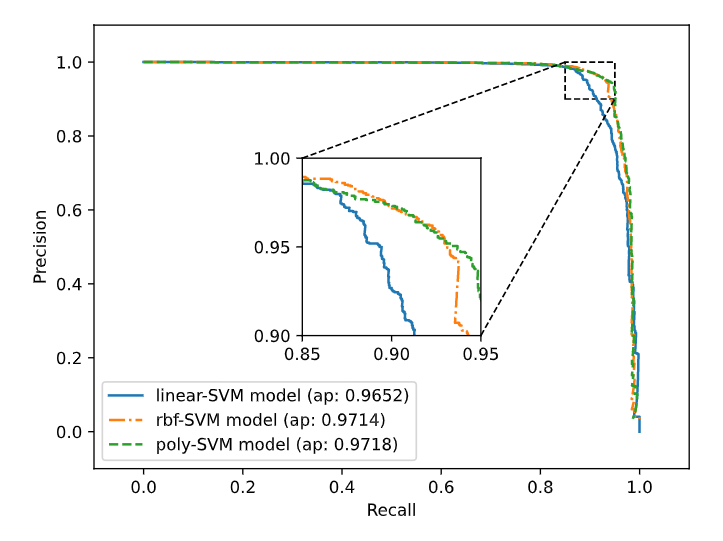
\includegraphics[scale=0.35]{Pics/SVM_prcurve_donor.png}
    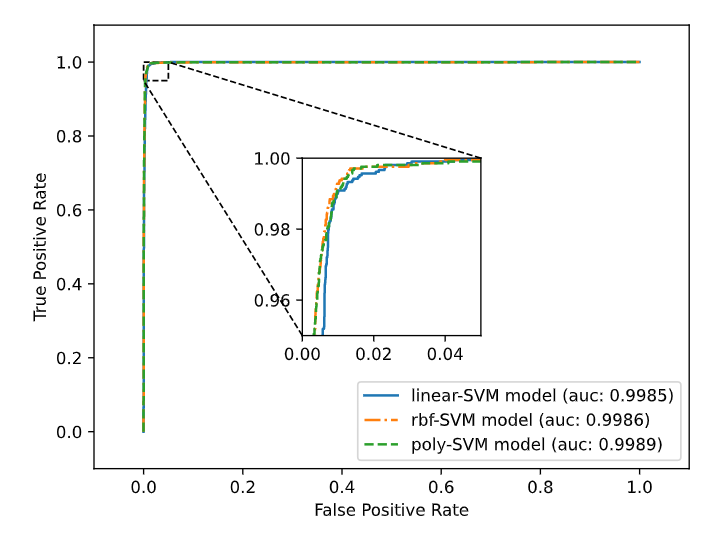
\includegraphics[scale=0.35]{Pics/SVM_roccurve_donor.png}}
\caption{Measuring SVM models on the BG set. \textbf{Left}: Precision-Recall curves plotted by using a bunch of thresholds. Average Precision is marked at the figure legend, which represents areas under the P-R curves. There is a larger performance gap between linear SVM and other 2 SVMs, which means that the distribution of splice site vectors are of poor linear-separability. \textbf{Right}: ROC curves with AUC marked at the figure legend, which represents areas under the ROC. All 3 SVMs behaved well on the given training data with impressive predicting precisions, in which 4D-poly SVM attaining an incredible AUC = 0.9989. The best $C_K$ , $\gamma$ and degree provided by grid searching are assigned to SVMs to get the best metrics. }
\label{fig3}
\end{figure*}

\begin{figure*}[htbp]
\centerline{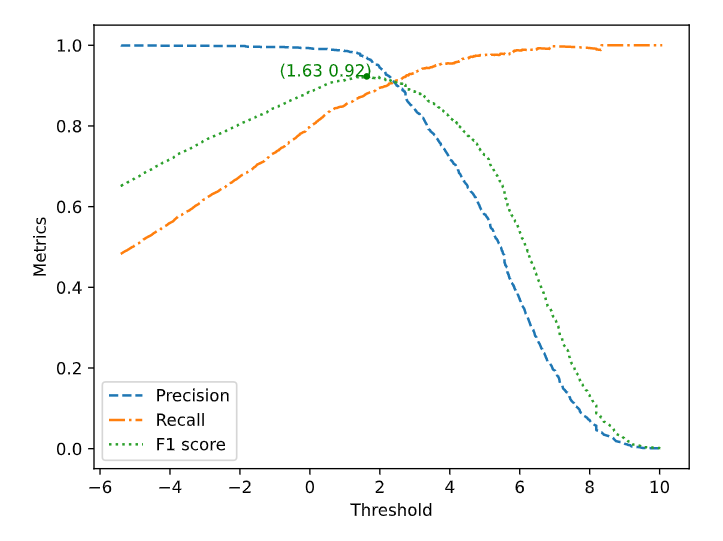
\includegraphics[scale=0.23]{Pics/linear-SVM_threshold_donor.png}
    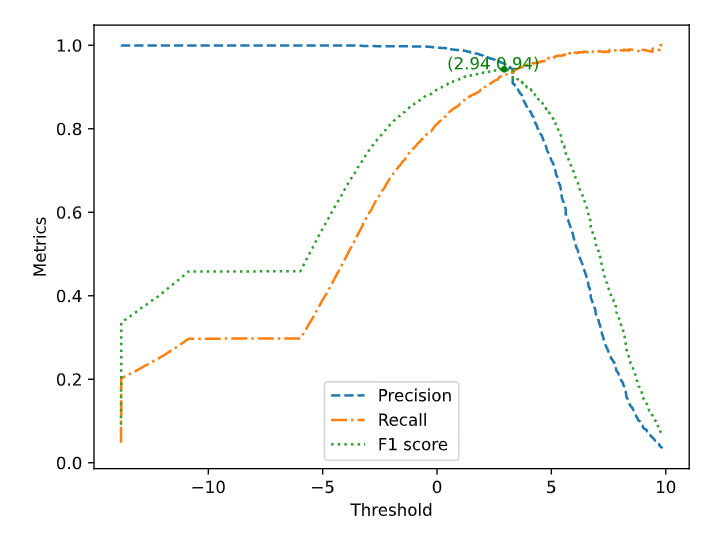
\includegraphics[scale=0.23]{Pics/rbf-SVM_threshold_donor.png}
    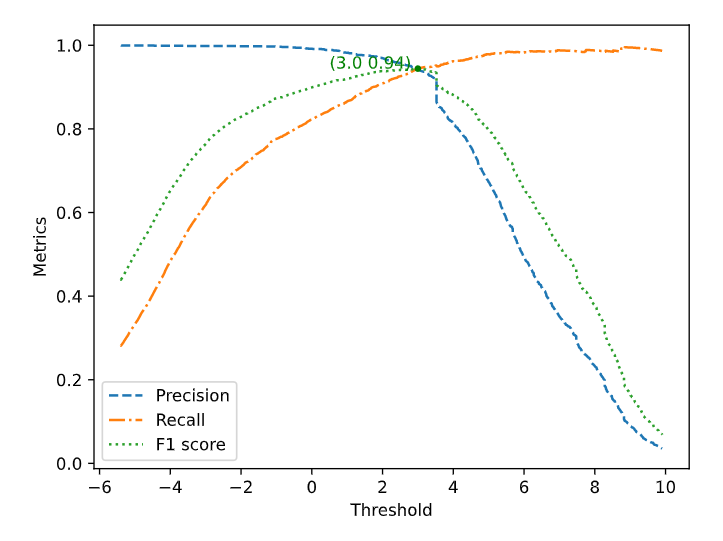
\includegraphics[scale=0.23]{Pics/poly-SVM_threshold_donor.png}}
\caption{Searching for the best thresholds for donor prediction. F1-score \eqref{eq10} is a balanced metric between  precision and recall which expresses best performance of models. We have found the maximum F1 points and values for all 3 SVMs: \textbf{left}, linear SVM, (1.63, 0.92); \textbf{center}, RBF SVM, (2.94, 0.94); \textbf{right}, 4D-poly SVM, (3.00, 0.94). }
\label{fig4}
\end{figure*}

\subsection{Implementation}\label{3.3}

We encapsulate the SVM model in the class \texttt{Svm} which is derived from the base class \texttt{Base} in \texttt{./Model/basemodel.py}. Sequences are extracted by \texttt{./Utils/extract.py} and saved temporarily in an \texttt{Sequence} object. All of the statistical graphs involved in this paper are drawn by the scripts in \texttt{./Utils} using Matplotlib \cite{Hunter:2007} and Weblogo, and saved in \texttt{./Pics}. We evaluate the model and search for the best parameters using Scikit-Learn for confusion matrices, precision-recall pairs and FPR-TPR pairs \cite{pedregosa2011scikit}. These tools saved considerable time for model training and prediction. Models can be easily saved or loaded by methods \texttt{save\_model()} and \texttt{load\_model()}. All the components have their corresponding interface methods provided in the aforementioned classes. For the code implementation details of SVM, see \texttt{./Model/wam.py}. 

Training \& Predicting process is operated by Ubuntu 18.04.5 LTS on 16 CPU cores with 2 threads each. It is highly recommended to use the optimized SVM module \texttt{thundersvm} instead of \texttt{sklearn.svm} for GPU support when CUDA 9.0 is available. The source code is available on GitHub and can be obtained from \url{https://github.com/Newiz430/SplicePredictor}. 

\begin{figure*}[htbp]
\centerline{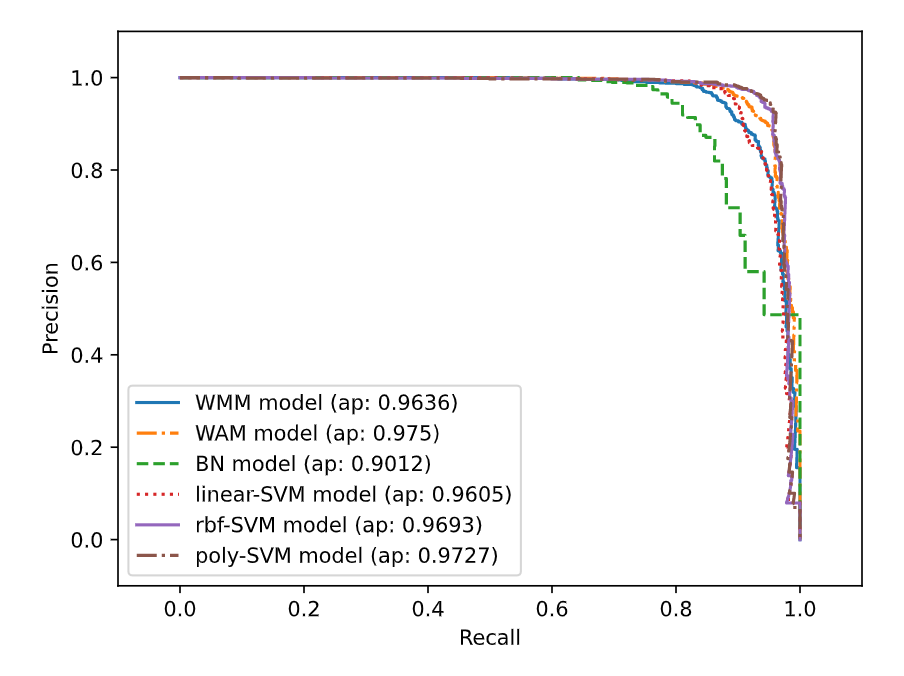
\includegraphics[scale=0.28]{Pics/all_prcurve_donor.png}
    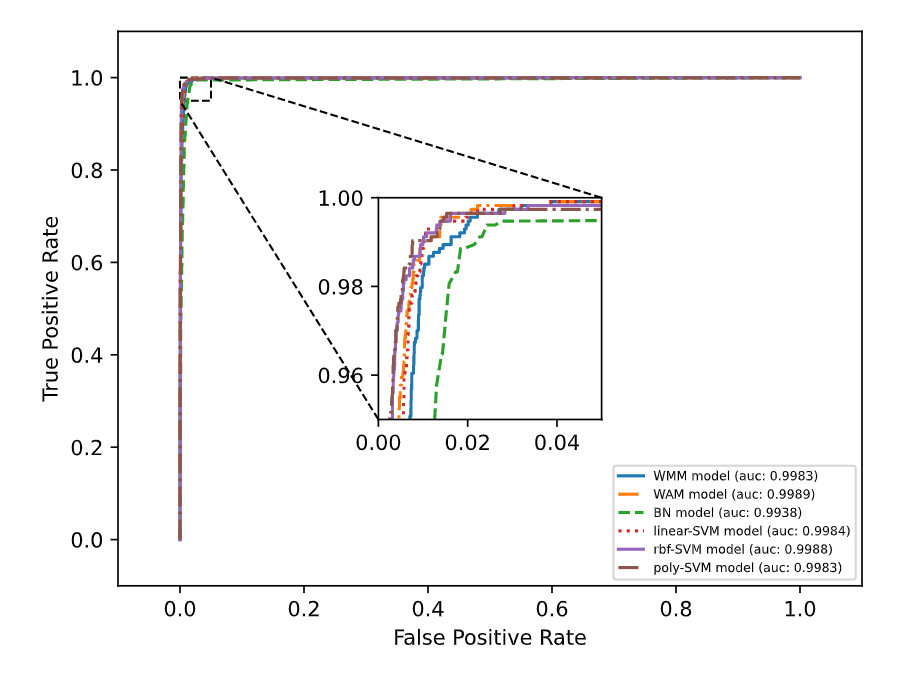
\includegraphics[scale=0.28]{Pics/all_roccurve_donor.png}}
\caption{Overall comparison of splice predictors: \textbf{left}, P-R curves; \textbf{right}, ROC curves. As we can see, RBF and 4D-polynomial SVM reaches the highest Precision-Recall points (about 0.93 both, see Table \ref{tab2}), although the average precisions are not the best. RBF SVM surpasses 4D-poly SVM on AUC by +0.0005 which cannot tell the difference between the predicting performance. Result given by linear SVM is acceptable as well, considering its lightweight computation. }
\label{fig5}
\end{figure*}

\section{Results}\label{4}

\subsection{Searching Suitable Parameters}\label{4.1}

Hyperparameters are crucial to model performance. To seek for the perfect parameters, we does a cross-validated exhaustive search \cite{hsu2003practical} over the kernels, $C_K$ and $\gamma$ using the donor samples. Results are shown in Table \ref{tab1}. See Appendix \ref{A} for detailed data. 

\begin{table}[htbp]
\begin{center}
\begin{threeparttable}
\caption{Results of Grid Searching on Hyperparameters of SVMs}
\begin{tabular}{lccc}
\toprule
Kernel & \tabincell{c}{Highest Mean Cross-\\validation Score} & Argmax($C_K$)\tnote{1} & Argmax($\gamma$) \\
\midrule
Linear & 0.9847 & 100 & \\
RBF (Gaussian) & 0.9885 & 10 & `scale' \\
2-D polynomial & 0.9888 & 1 & `scale' \\
3-D polynomial & 0.9889 & 1 & `scale' \\
4-D polynomial & \textbf{0.9894} & 1 & `scale' \\
\bottomrule
\end{tabular}
\begin{tablenotes}
    \footnotesize
    \item[1] If there are multiple $C_K$ or $\gamma$ with the same cross-validation score, $C_K$ in the table is by default the valid minimum.  
\end{tablenotes}
\label{tab1}
\end{threeparttable}
\end{center}
\end{table}

We found that data standardization cause a manifest reduction of grid searching efficiency. Under the same experimental condition, the number of iterations for each optimization process on scaled data  increased a hundredfold compared to the original one-hot data, hence we abandoned data standardization throughout the grid searching. 

With the best parameters we obtained, we evaluated 3 models with different kernels by P-R curves and ROC curves. From our results in Fig. \ref{fig3}, we came up to a conclusion that 4-D polynomial SVM fits the best for donor site predicting tasks.  

\begin{table*}[htbp]
\begin{center}
\begin{threeparttable}
\caption{Performance of SVMs Against Other Donor Site Predictors\tnote{1}}
\begin{tabular}{lccccc}
\toprule
Method & Precision & Recall (TPR) & FPR & F1-score & Run time(s) \\
\midrule
WMM (threshold = 2.26) & 0.8503 & \textbf{0.9697} & 0.0085 & 0.9061 & \textbf{1.6614} \\
WAM (threshold = 3.09) & 0.9006 & 0.9543 & 0.0053 & 0.9267 & 1.7940 \\
BN (threshold = 2.32) & 0.8067 & 0.9410 & 0.0113 & 0.8688 & 4.23e+3 \\
Linear - SVM (threshold = 1.63) & 0.8801 & 0.9678 & 0.0066 & 0.9219 & 2.3974 \\
RBF - SVM (threshold = 2.94) & 0.9265 & 0.9278 & 0.0037 & 0.9272 & 3.4894 \\
4D poly - SVM (threshold = 3.00) & \textbf{0.9290} & 0.9384 & \textbf{0.0036} & \textbf{0.9337} & 3.0368 \\
\bottomrule
\end{tabular}
\begin{tablenotes}
    \footnotesize
    \item[1] The argmax thresholds are assigned to these models to get the best metrics. Run time represents the seconds cost in the predicting step. Same for tables below. 
\end{tablenotes}
\label{tab2}
\end{threeparttable}
\end{center}
\end{table*}

\subsection{Donor Site Prediction}\label{4.2}

\emph{Comparison studies. } Here we summarize the performance of various splice site predicting models such as WMM, WAM, Bayesian network and our proposed models. The results in Fig. \ref{fig5} show that our work achieves prominent accuracy on splice site predicting tasks. 

We used the training set of the same size and predicting procedure for both two models, and performed them on the same set of testing data with the best threshold Fig. \ref{fig6} pointing out. In Table \ref{tab1}, we present the stats of accuracy for both models. It indicates that WAM improves the overall signal predicting effect within an approximate predicting time. WAM shows a +2.27\% improvement on F1-score from 0.9061 up to 0.9267. 

We present the stats of accuracy for all evaluated models in Table \ref{tab2}. It indicates that both RBF and 4D-polynomial SVM improves the predicting result and the latter achieves the best performance among all models. 4D-polynomial SVM shows an outstanding improvement on F1-score up to 0.9337 which, more than that, predicts slightly faster than its biggest competitor - RBF SVM. In general, SVMs sacrifice a little amount of time for an improvement of accuracy, which is totally worthwhile. 

\begin{figure*}[htbp]
\centerline{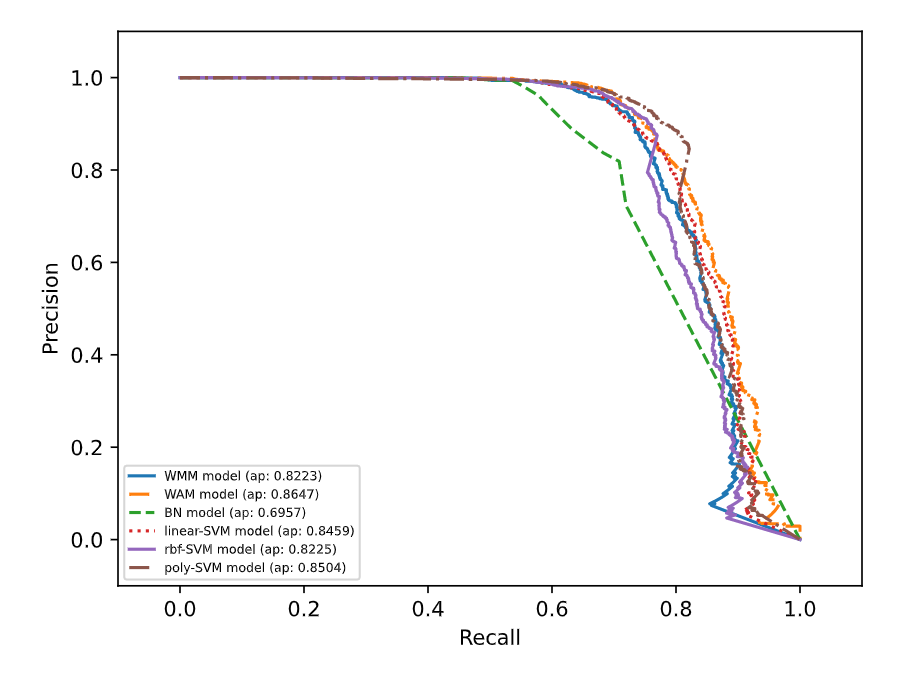
\includegraphics[scale=0.28]{Pics/all_prcurve_acceptor.png}
    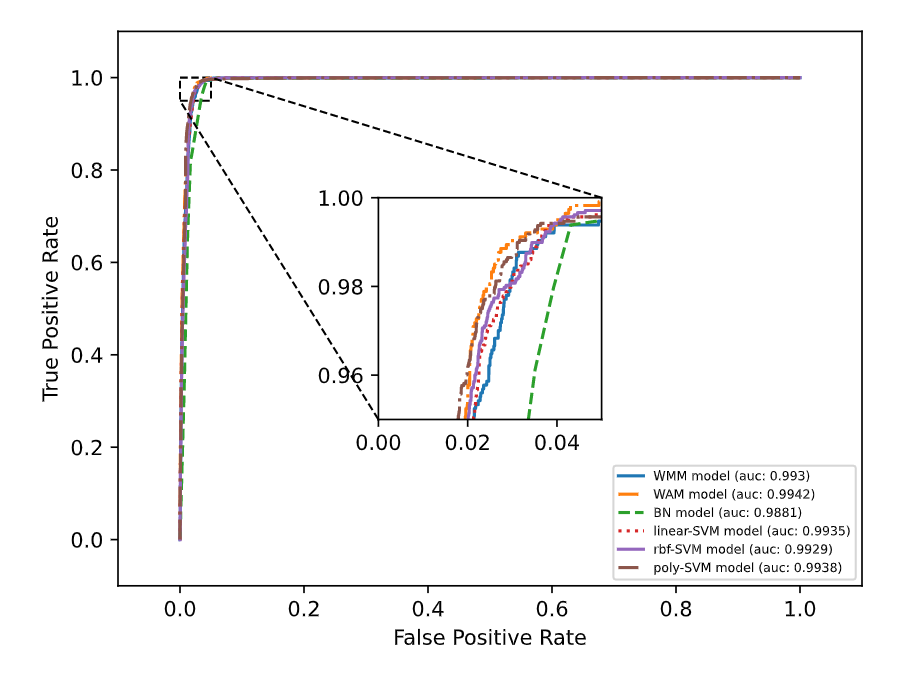
\includegraphics[scale=0.28]{Pics/all_roccurve_acceptor.png}}
\caption{Precision-Recall curves (\textbf{left}) and ROC curves (\textbf{right}) for acceptor signal. SVMs used for acceptor seems to have a lower predicting ability relative to the one for donor. Besides, linear SVM gives a better result than RBF ones, which is still not prominent. }
\label{fig6}
\end{figure*}

\begin{figure*}[htbp]
\centerline{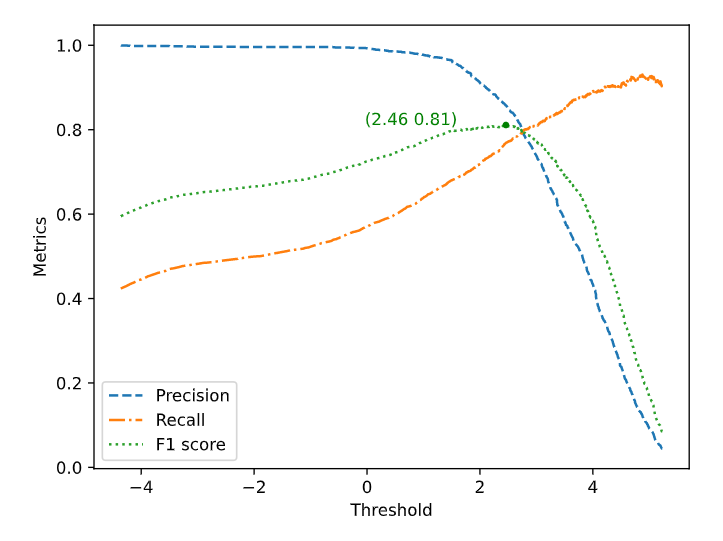
\includegraphics[scale=0.23]{Pics/linear-SVM_threshold_acceptor.png}
    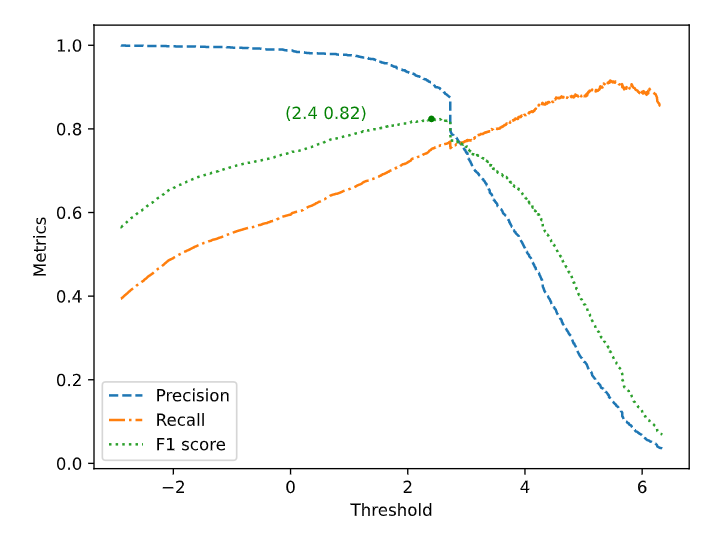
\includegraphics[scale=0.23]{Pics/rbf-SVM_threshold_acceptor.png}
    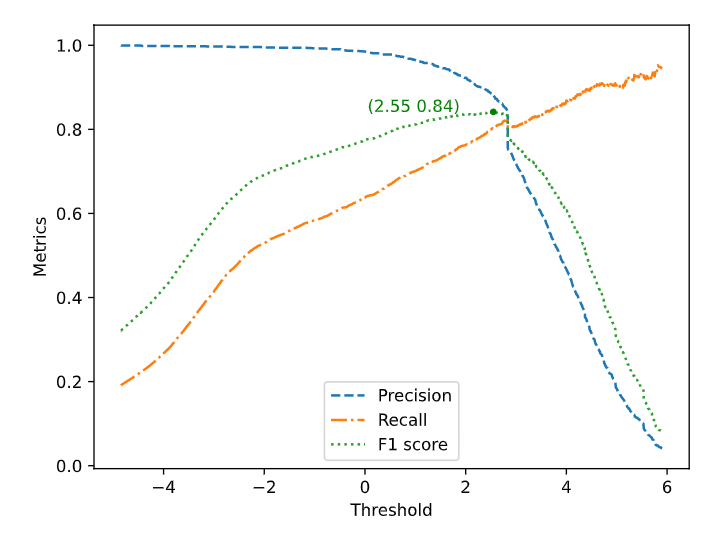
\includegraphics[scale=0.23]{Pics/poly-SVM_threshold_acceptor.png}}
\caption{Searching for the best thresholds for acceptor prediction. We have found the maximum F1 points and values for all 3 SVMs: \textbf{left}, linear SVM, (2.46, 0.81); \textbf{center}, RBF SVM, (2.40, 0.82); \textbf{right}, 4D-poly SVM, (2.55, 0.84). }
\label{fig7}
\end{figure*}

\subsection{Acceptor Site Prediction}\label{4.3}

We did the same experiment on acceptor sites. Consequences are displayed in Fig. \ref{fig6} -- \ref{fig7} and Table \ref{tab3}. We make a hypothesis that the best coefficients provided by the grid searching in section \ref{4.1} are also ideal for acceptor predictors, which is reasonable since the number and quality of donor and acceptor sites is identical. 4D polynomial SVM, likewise, achieves the best performance among all predictors as expected. 

\begin{table*}[htbp]
\begin{center}
\begin{threeparttable}
\caption{Performance of SVMs Against Other Acceptor Site Predictors}
\begin{tabular}{lccccc}
\toprule
Method & Precision & Recall (TPR) & FPR & F1-score & Run time(s) \\
\midrule
WMM (threshold = 2.69) & 0.7385 & \textbf{0.9038} & 0.0160 & 0.8128 & \textbf{1.3336} \\
WAM (threshold = 2.54) & 0.7554 & \textbf{0.9038} & 0.0146 & 0.8229 & 1.4286 \\
BN (threshold = 3.38) & 0.7083 & 0.8187 & 0.0169 & 0.7595 & 1.02e+3 \\
Linear - SVM (threshold = 2.46) & 0.7603 & 0.8653 & 0.0137 & 0.8094 & 2.5636 \\
RBF - SVM (threshold = 2.40) & 0.7677 & 0.8999 & 0.0136 & 0.8285 & 4.6039 \\
4D poly - SVM (threshold = 2.55) & \textbf{0.7774} & 0.8975 & \textbf{0.0129} &  \textbf{0.8331} & 3.3924 \\
\bottomrule
\end{tabular}
\label{tab3}
\end{threeparttable}
\end{center}
\end{table*}

\section{Discussion}

Overall, we formulate and re-implement an application of SVM model by training it on the Kulp \& Reese dataset. We find the perfect hyperparameters to fit an optimum hyperplane and compare its performance against other feasible approaches, successfully proving its superiority on the accuracy and efficiency of predicting donor \& acceptor splice sites. 

As a matter of fact, there are still some blemishes in our methods which need to be taken serious consideration. We only sampled a fraction of data for SVM learning thus our model may not attain its best performance with the given training set. We ignored the odds of base indels in signal sequences. We omitted unambiguous bases at the beginning of our work which is likely to be part of the splice site patterns. GPU has not been used for acceleration so SVM predicting speed still has a huge promotion space. What's more, we only tried one single feature selection tactic limited by the deadline (our model is actually designed for feature sequences of different lengths as input). 

In the future, we will try to improve the performance of SVM by optimizing the architecture of training set, and apply SVM on more tasks about sequence pattern recognition, aside from addressing the issues above. 

\section*{Acknowledgment}

This work was supported by Prof. Zhou from College of Life Science \& Technology, Huazhong University of Science and Technology, and Wuhan National Laboratory for Optoelectronics for providing computing resources. Also acknowledge our classmates for helpful suggestions \& corrections. 

\bibliographystyle{unsrt}
\bibliography{references}

\vspace{9cm}

\appendices
\section{Hyperparameter Searching}\label{A}

An exhaustive search on the coefficients of donor SVM is applied during our experiment. We set the grid as: Kernels, (Linear, RBF, 2-D polynomial, 3-D polynomial, 4-D polynomial); $C_K$, (1, 10, 100, 1,000, 10,000); $\gamma$, (0.001, 0.01, 0.1, 1, auto: 1 / n\_features, scale: 1 / (n\_features * \texttt{X.var()}) with \texttt{X.var()} for the variance of unscaled data. Results are shown below. 

\begin{table}[htbp]
\begin{center}
\caption{Grid Searching Results for Linear SVM}
\begin{tabular}{|c|c|}
\hline
$C_K$ & Mean Cross-validation Score \\
\hline
1 & 0.98319994 \\
10 & 0.98441918 \\
100 & \textbf{0.98469027} \\
1,000 & \textbf{0.98469027} \\
10,000 & \textbf{0.98469027} \\
\hline
\end{tabular}
\label{tab4}
\end{center}
\end{table}

\clearpage

\begin{table*}[tbp]
\begin{center}
\caption{Grid Searching Results for RBF SVM}
\begin{tabular}{|c|cccccc|}
\hline
\diagbox{$C_K$}{$\gamma$} & 0.001 &0.01 & 0.1 & 1 & auto & scale \\
\hline
1 & 0.97032906 & 0.97574838 & 0.98590969 & 0.84974909 & 0.98238657 & 0.98712866 \\
10 & 0.97547737 & 0.98319985 & 0.98645142 & 0.84974909 & 0.98780607 & \textbf{0.98848358} \\
100 & 0.98238693 & 0.98685774 & 0.98469009 & 0.84974909 & 0.98821267 & 0.98726416 \\
1,000 & 0.98550328 & 0.98441900 & 0.98469009 & 0.84974909 & 0.98455431 & 0.98726416 \\
10,000 & 0.98685774 & 0.97967709 & 0.98469009 & 0.84974909 & 0.98455431 & 0.98726416 \\
\hline
\end{tabular}
\label{tab5}
\end{center}
\end{table*}

\begin{table*}[tbp]
\begin{center}
\caption{Grid Searching Results for 2-D Polynomial SVM}
\begin{tabular}{|c|cccccc|}
\hline
\diagbox{$C_K$}{$\gamma$} & 0.001 &0.01 & 0.1 & 1 & auto & scale \\
\hline
1 & 0.60659581 & 0.97561297 & 0.98631620 & 0.97859317 & 0.98143842 & \textbf{0.98875449} \\
10 & 0.92846226 & 0.98021937 & 0.98523191 & 0.97561278 & 0.98509641 & 0.98658702 \\
100 & 0.97561297 & 0.98631620 & 0.97859317 & 0.97561278 & 0.98767075 & 0.98184484 \\
1,000 & 0.98021937 & 0.98523191 & 0.97561278 & 0.97561278 & 0.98360590 & 0.98184484 \\
10,000 & 0.98631620 & 0.97859317 & 0.97561278 & 0.97561278 & 0.98184484 & 0.98184484 \\
\hline
\end{tabular}
\label{tab6}
\end{center}
\end{table*}

\begin{table*}[tbp]
\begin{center}
\caption{Grid Searching Results for 3-D Polynomial SVM}
\begin{tabular}{|c|cccccc|}
\hline
\diagbox{$C_K$}{$\gamma$} & 0.001 &0.01 & 0.1 & 1 & auto & scale \\
\hline
1 & 0.60659581 & 0.76098855 & 0.98699334 & 0.98401277 & 0.98468972 & \textbf{0.98889008} \\
10 & 0.60659581 & 0.98076156 & 0.98509659 & 0.98401277 & 0.98441881 & 0.98590924 \\
100 & 0.32258497 & 0.98252244 & 0.98401277 & 0.98401277 & 0.98916108 & 0.98550273 \\
1,000 & 0.87982323 & 0.98699334 & 0.98401277 & 0.98401277 & 0.98618024 & 0.98550273 \\
10,000 & 0.98076156 & 0.98509659 & 0.98401277 & 0.98401277 & 0.98550273 & 0.98550273 \\
\hline
\end{tabular}
\label{tab7}
\end{center}
\end{table*}

\begin{table*}[tbp]
\begin{center}
\caption{Grid Searching Results for 4-D Polynomial SVM}
\begin{tabular}{|c|cccccc|}
\hline
\diagbox{$C_K$}{$\gamma$} & 0.001 &0.01 & 0.1 & 1 & auto & scale \\
\hline
1 & 0.60659581 & 0.60659581 & 0.98739984 & 0.98496109 & 0.88551227 & \textbf{0.98943209} \\
10 & 0.60659581 & 0.60686672 & 0.98523210 & 0.98496109 & 0.98861890 & 0.98753516 \\
100 & 0.32258497 & 0.98509678 & 0.98496109 & 0.98496109 & 0.98794176 & 0.98753516 \\
1,000 & 0.32258497 & 0.98523255 & 0.98496109 & 0.98496109 & 0.98875458 & 0.98753516 \\
10,000 & 0.60659581 & 0.98739984 & 0.98496109 & 0.98496109 & 0.98753516 & 0.98753516 \\
\hline
\end{tabular}
\label{tab8}
\end{center}
\end{table*}

\end{document}
